%class
	\documentclass{beamer}

%template
	\usetheme{HannoverSalman}
	\setbeamertemplate{navigation symbols}{}
	%\setbeamertemplate{footline}{\centering{\insertframenumber/\insertpresentationendpage}}
	%\setbeamertemplate{footline}{\hspace*{.5cm}\scriptsize{\hfill\insertframenumber\hspace*{.5cm}}} 


%packages
	\usepackage{amsmath, amssymb, graphicx,cancel}
	\usepackage[absolute,overlay]{textpos}
	\usepackage{subfigure}
	\usepackage{caption}\captionsetup{labelformat=empty,labelsep=none}
	\usepackage{geometry}
	\geometry{verbose}
	\usepackage{color}
	\usepackage{xmpmulti}
	\usepackage[3D]{movie15}
	\usepackage{hyperref}
%	\usepackage{bookmark}
	\usepackage[open,openlevel=4,atend]{bookmark}
	%\bookmarksetup{color=blue}
	\usepackage{multirow}
	\usepackage[style=numeric,defernumbers, authoryear]{biblatex}
	%\usepackage[square,sort]{natbib}
	%\usepackage{fancyhdr}%\pagestyle{fancy} 

	
	\hypersetup{bookmarksdepth = 4}


%citations files
	\bibliography{MyCitations}

%logoCSIPCPL
    \setlength{\TPHorizModule}{1mm}
    \setlength{\TPVertModule}{1mm}
    \newcommand{\logoCSIPCPL}
    {
    	\begin{textblock}{1}(100,2) %(100,85)  for bottom
    		
\includegraphics[width=1.5cm]{figs/logo_CSIP}
    	\end{textblock}
    	
	\begin{textblock}{1}(117,1) %(117,85)  for bottom
    		
\includegraphics[width=1.0cm]{figs/logo_CPL}
    	\end{textblock} 
    }

%logo evolution
    \newcommand{\logoEvolution}
    {    	
	\begin{textblock}{1}(110,1) %(117,85)  for bottom
    		\includegraphics[width=0.65in]{figs/logo_evolution.pdf}
    	\end{textblock} 
    }

%logo Qualcomm
    \newcommand{\logoQualcomm}
    {
    	\begin{textblock}{1}(110,2) %(100,85)  for bottom
    		\includegraphics[width=1.5cm]{figs/logo_qualcomm.jpg}
    	\end{textblock}
    }
%logo Qualcomm (long)
    \newcommand{\logoQualcommllong}
    {
    	\begin{textblock}{1}(0,0) 
    		\includegraphics[width=1.25in]{figs/logo_qualcomm_long.jpg}
    	\end{textblock}
    }

%logo Tech Tower
    \newcommand{\logoTechTower}
    {
    	\begin{textblock}{1}(0,0) 
    		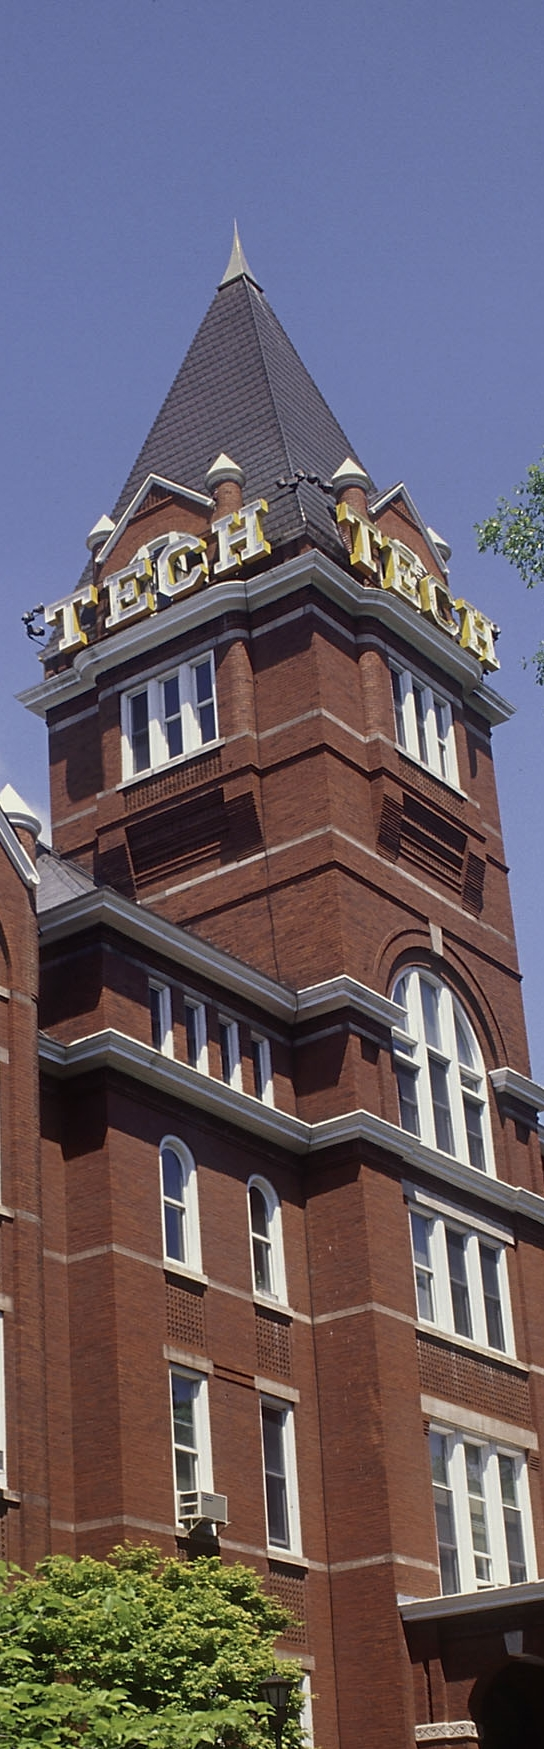
\includegraphics[width=1.25in]{figs/logo_TechTower.jpg}
    	\end{textblock}
    }

%logo tree
    \newcommand{\logoTree}
    {
    	\begin{textblock}{1}(0,0) 
    		\includegraphics[width=1.25in]{figs/logo_tree.jpg}
    	\end{textblock}
    }
%page numbers
    \newcommand{\mypagenum}
    {
    	\begin{textblock}{1}(1,94) 
		{\tiny \color[rgb]{0.2,0.2,1}\insertframenumber} %\insertframenumber,\insertpresentationendpage, \inserttotalframenumber
    	\end{textblock}
    }
%my footnote citation
	\newcommand{\myFootnoteCitation}[2]
	{
		\footnote{\tiny \citeauthor{#1}, \emph{#2}, \citeyear{#1}.}  %\citeauthor{#1}, \citetitle{#1}, #2 \citeyear{#1}.
	}
%my refer to citation
	\newcommand{\mycite}[1]
	{
		\emph{\citeauthor{#1} (\citeyear{#1})}
	}
%my footnote website citation
	\newcommand{\myFootnoteWebsiteCitation}[1]
	{
		\footnote{\tiny \citeauthor{#1}}
	}

\let\thefootnote\relax\footnotetext{Footnotetext without footnote mark}


%section underline
%\newcommand{\tmpsection}[1]{}
%\let\tmpsection=\section
%\renewcommand{\section}[1]{\tmpsection{\underline{#1}}}



%commands
	\newcommand{\likelihood}{p(Z_k| x_k) }						%likelihood
	\newcommand{\prior}{p(x_k)  } 								%prior
	\newcommand{\posterior} {p(x_k| Z_k)}						%posterior
	\newcommand{\prediction} {p(x_k| Z_{k-1})}					%prediction
	\newcommand{\update} {p(x_k|Z_k)}							%update
	\newcommand{\observations} {p(Z_k)}						%observations
	\newcommand{\prevobservations} {p(Z_{k-1})}				%previous observations
	\newcommand{\dxpk} {dx_{k-1}}							%dx_{k-1}
	\newcommand{\ChapKolm}{\int{p(x_k| x_{k-1})p(x_{k-1}|Z_{k-1})} \dxpk} %Chapman Kolmogorov

	%algorithm specific: JPDAF
	\newcommand{\likelihoodJPDAF}{p(Z_k| \chi, m, Z_{k-1}) }		%1. likelihood
	\newcommand{\priorJPDAF}{p(\chi|m, Z^{k-1}} 				%2. prior	
	\newcommand{\observationsJPDAF} {p(Z_k}					%3. observations
	\newcommand{\posteriorJPDAF} {p(\chi| Z_k)}					%4. posterior

%environments
	\newenvironment{changemargin}[2]
	{
	  	\begin{list}{}
		{
			\setlength{\topsep}{0pt}%
			\setlength{\leftmargin}{#1}%
			\setlength{\rightmargin}{#2}%
			\setlength{\listparindent}{\parindent}%
			\setlength{\itemindent}{\parindent}%
			\setlength{\parsep}{\parskip}%
		}
	  	\item[]
		}
		{\end{list}
	}
%figures

%colors
\definecolor{darkgreen}{rgb}{0,0.5,0}

%personal details
	\author{Salman Aslam}
	\institute{Advisor, Dr Christopher Barnes (ECE)\\Co-advisor, Dr Aaron Bobick (CoC)\\Georgia Institute of Technology}
	\date{}

\begin{document}
%####################################################################################################
\title{Visual Tracking \\ (appearance)}
%####################################################################################################
\begin{frame}[plain]\logoTechTower
	\titlepage
\end{frame}

\begin{frame}
\frametitle{Outline}
\logoCSIPCPL\logoTechTower
	\setcounter{tocdepth}{1}	
	\tableofcontents
\end{frame}

%#######################################################################
\section{INTRODUCTION}
%#######################################################################
\begin{frame}
\frametitle{Introduction}
\framesubtitle{overview}
\logoCSIPCPL\mypagenum
	\begin{enumerate}
		\item Template matching
			\begin{itemize}
				\item fixed templates: reliable over short durations
			\end{itemize}
		\item Subspace methods
			\begin{itemize}
				\item usually learned with PCA
				\item model variations in lighting and pose
				\item disadvantages: object specific, training
			\end{itemize}			
		\item Probability density
			\begin{itemize}
				\item robustness under image distortions and occlusions
				\item fast to learn
				\item disadvantage: lack of expressiveness, registration can be difficult
			\end{itemize}
		\item Motion
			\begin{itemize}
				\item optical flow works well for small displacements
				\item block matching for large motion
				\item computing motion vectors is computationally complex
			\end{itemize}
	\end{enumerate}
\end{frame}


\begin{frame}
\frametitle{Introduction}
\framesubtitle{template matching}
\logoCSIPCPL\mypagenum
	\begin{itemize}
		\item Templates tend to become stale over time
	\end{itemize}
	\href{run:distribute/run_TRK_templateMatching.bat}{{\color{blue}\underline {Template matching}}}
\end{frame}

%#######################################################################
\section{PRIOR WORK}
%#######################################################################
%=================================
\subsection{1996: illum./geometry (Hallinan)}
%=================================
\begin{frame}
\frametitle{Prior work: illumination and geometry}
\framesubtitle{5. methodology}
\logoCSIPCPL\mypagenum
\myFootnoteCitation{1994_TRK_subspace_Hallinan}{CVPR}
	\begin{itemize}
		\item illumination: basis functions
		\item geometry: warping
	\end{itemize}
\end{frame}



\begin{frame}
\frametitle{Prior work: illum./geometry (Hallinan)}
\framesubtitle{7. general points}
\logoCSIPCPL\mypagenum
\myFootnoteCitation{1994_TRK_subspace_Hallinan}{CVPR}
	\begin{itemize}
		\item SSD-based tracking methods tend to concentrate on handling geometry 
			\begin{itemize}
				\item most implementations of SSD tracking only solve for a rigid translation of the target region
			\end{itemize}
	\end{itemize}
\end{frame}




%=================================
\subsection{1998: IIR templates (Lipton)}
%=================================
\begin{frame}
\frametitle{Prior work: template matching}
\framesubtitle{1. overview}
\mypagenum
\myFootnoteCitation{1998_CNF_Tracking_Lipton}{WACV}
	\begin{figure}
		\includegraphics[width=1.0\textwidth]{tables/TrackingPapers_AppearanceTracking_1998_Lipton.pdf}
	\end{figure}
\end{frame}



\begin{frame}
\frametitle{Prior work: IIR templates (Lipton)}
\framesubtitle{5. methodology}
\logoCSIPCPL\mypagenum
\myFootnoteCitation{1998_CNF_Tracking_Lipton}{WACV}
	\begin{itemize}
		\item tracking process involves correlation matching between a template and the current motion region (obtained by DT, i.e. temporal differencing)
		\item the motion region with the best correlation is tracked and is used to update the template for subsequent tracking
		\item template update is done using 	
		\begin{equation*}
			R_n = \alpha M_n + (1- \alpha)R_{n-1}
		\end{equation*}
		here $M_n$ is the motion region, i.e. current template
	\end{itemize}
\end{frame}


\begin{frame}
\frametitle{Prior work: IIR templates (Lipton)}
\framesubtitle{7. general points}
\logoCSIPCPL\mypagenum
\myFootnoteCitation{1998_CNF_Tracking_Lipton}{WACV}
	\begin{figure}
		\includegraphics[width=0.7\textwidth]{tables/TrackingPapers_AppearanceTracking_1998_Lipton_DTvsTM.pdf}
	\end{figure}
	\begin{itemize}
		\item Kalman filter of limited use since based on unimodal Gaussian densities and hence cannot support simultaneous alternative motion hypotheses
	\end{itemize}
\end{frame}





\begin{frame}
\frametitle{Prior work: IIR templates (Lipton)}
\framesubtitle{figures}
\mypagenum
\myFootnoteCitation{1998_CNF_Tracking_Lipton}{WACV}
	\begin{figure}
		\includegraphics[height=0.75\textheight]{figs/TrackingPapers_template_1998_Lipton_fig1.jpg}
	\end{figure}
\end{frame}


\begin{frame}
\frametitle{Prior work: IIR templates (Lipton)}
\framesubtitle{figures (cont.)}
\mypagenum
\myFootnoteCitation{1998_CNF_Tracking_Lipton}{WACV}
	\begin{figure}
		\includegraphics[width=1.0\textwidth]{figs/TrackingPapers_template_1998_Lipton_fig2.jpg}
	\end{figure}
\end{frame}


\begin{frame}
\frametitle{Prior work: IIR templates (Lipton)}
\framesubtitle{figures (cont.)}
\mypagenum
\myFootnoteCitation{1998_CNF_Tracking_Lipton}{WACV}
	\begin{figure}
		\includegraphics[width=1.0\textwidth]{figs/TrackingPapers_template_1998_Lipton_fig3.jpg}
	\end{figure}
\end{frame}



\begin{frame}
\frametitle{Prior work: IIR templates (Lipton)}
\framesubtitle{figures (cont.)}
\mypagenum
\myFootnoteCitation{1998_CNF_Tracking_Lipton}{WACV}
	\begin{figure}
		\includegraphics[width=1.0\textwidth]{figs/TrackingPapers_template_1998_Lipton_fig4.jpg}
	\end{figure}
\end{frame}



\begin{frame}
\frametitle{Prior work: IIR templates (Lipton)}
\framesubtitle{figures (cont.)}
\mypagenum
\myFootnoteCitation{1998_CNF_Tracking_Lipton}{WACV}
	\begin{figure}
		\includegraphics[height=0.75\textheight]{figs/TrackingPapers_template_1998_Lipton_fig5.jpg}
	\end{figure}
\end{frame}



\begin{frame}
\frametitle{Prior work: IIR templates (Lipton)}
\framesubtitle{figures (cont.)}
\mypagenum
\myFootnoteCitation{1998_CNF_Tracking_Lipton}{WACV}
	\begin{figure}
		\includegraphics[height=0.75\textheight]{figs/TrackingPapers_template_1998_Lipton_fig6.jpg}
	\end{figure}
\end{frame}



\begin{frame}
\frametitle{Prior work: IIR templates (Lipton)}
\framesubtitle{figures (cont.)}
\mypagenum
\myFootnoteCitation{1998_CNF_Tracking_Lipton}{WACV}
	\begin{figure}
		\includegraphics[height=0.75\textheight]{figs/TrackingPapers_template_1998_Lipton_fig7.jpg}
	\end{figure}
\end{frame}



\begin{frame}
\frametitle{Prior work: IIR templates (Lipton)}
\framesubtitle{figures (cont.)}
\mypagenum
\myFootnoteCitation{1998_CNF_Tracking_Lipton}{WACV}
	\begin{figure}
		\includegraphics[height=0.75\textheight]{figs/TrackingPapers_template_1998_Lipton_fig8.jpg}
	\end{figure}
\end{frame}



\begin{frame}
\frametitle{Prior work: IIR templates (Lipton)}
\framesubtitle{figures (cont.)}
\mypagenum
\myFootnoteCitation{1998_CNF_Tracking_Lipton}{WACV}
	\begin{figure}
		\includegraphics[height=0.75\textheight]{figs/TrackingPapers_template_1998_Lipton_fig9.jpg}
	\end{figure}
\end{frame}



\begin{frame}
\frametitle{Prior work: IIR templates (Lipton)}
\framesubtitle{figures (cont.)}
\mypagenum
\myFootnoteCitation{1998_CNF_Tracking_Lipton}{WACV}
	\begin{figure}
		\includegraphics[height=0.75\textheight]{figs/TrackingPapers_template_1998_Lipton_fig10.jpg}
	\end{figure}
\end{frame}



\begin{frame}
\frametitle{Prior work: IIR templates (Lipton)}
\framesubtitle{figures (cont.)}
\mypagenum
\myFootnoteCitation{1998_CNF_Tracking_Lipton}{WACV}
	\begin{figure}
		\includegraphics[width=1.0\textwidth]{figs/TrackingPapers_template_1998_Lipton_table1.jpg}
	\end{figure}
\end{frame}


%=================================
\subsection{2000: deform. templates (Zhong)}
%=================================
\begin{frame}
\frametitle{Prior work: deform. templates (Zhong)}
\framesubtitle{figures}
\mypagenum
\myFootnoteCitation{2000_JNL_TRK_region_Zhong}{PAMI}
	\begin{figure}
		\includegraphics[height=0.75\textheight]{figs/TrackingPapers_deformableTemplates_2000_Zhong_fig3.jpg}
	\end{figure}
\end{frame}





%=================================
\subsection{2003: adaptive appearance (Jepson)}
%=================================
\begin{frame}
\frametitle{Prior work: adaptive appearance (Jepson)}
\framesubtitle{1. overview}
\mypagenum
\myFootnoteCitation{2003_JNL_TRKsubspace_Jepson}{PAMI}
	\begin{figure}
		\includegraphics[width=1.0\textwidth]{tables/TrackingPapers_SubspaceTracking_2003_AdaptiveAppearance.pdf}
	\end{figure}

\end{frame}


\begin{frame}
\frametitle{Prior work: adaptive appearance (Jepson)}
\framesubtitle{2. summary}
\mypagenum
\myFootnoteCitation{2003_JNL_TRKsubspace_Jepson}{PAMI}
	\begin{itemize}
		\item adaptive phase-based appearance model	
		\item goal is to get optimal image warp from the stable properties of image appearance
		\item 3 components
			\begin{itemize}
				\item $\mathcal{W}$: wandering component, tracking portion (gaussian density)
				\item $\mathcal{S}$: stable model, captures behavior of temporally stable and slowly varying image observations, when and where they occur (gaussian density)
				\item $\mathcal{L}$: lost component, data outliers (uniform density), 
			\end{itemize}
		\item these 3 are combined into a probabilistic mixture model (generative)
	\end{itemize}
\end{frame}


\begin{frame}
\frametitle{Prior work: adaptive appearance (Jepson)}
\framesubtitle{figures}
\mypagenum
\myFootnoteCitation{2003_JNL_TRKsubspace_Jepson}{PAMI}
	\begin{figure}
		\includegraphics[width=1.0\textwidth]{figs/TrackingPapers_descriptors_2003_Jepson_fig5.jpg}
	\end{figure}
\end{frame}







%=================================
\subsection{2008: OpenCV book (Bradski)}
%=================================
\begin{frame}
\frametitle{Prior work: OpenCV book (Bradski)}
\framesubtitle{figures}
\mypagenum
\myFootnoteCitation{2008_BOOK_OpenCV_Bradski}{O'Reilly}
	\begin{figure}
		\includegraphics[height=0.5\textheight]{figs/Books_OpenCV_1998_Bradski_fig7_11.jpg}
	\end{figure}
	\begin{itemize}
		\item in outdoor images, better to use normalized method (i.e. 0 to 1 output)
		\item correlation coefficient works best in above example, but at greater computational cost
	\end{itemize}
\end{frame}


%####################################################################################################
\printbibliography
%####################################################################################################
%\bibliographystyle{ieee}
%\bibliography{c:/salman/work/writing/MyCitations}
\end{document}
%####################################################################################################

%####################################################################################################
